\usebeamerfont{block body}

\begin{figure}
  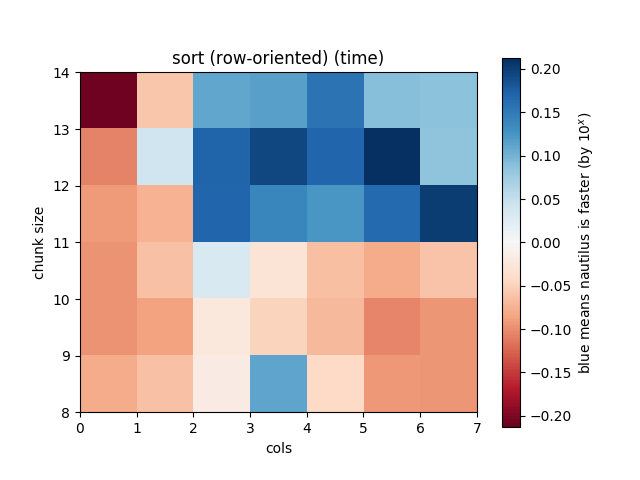
\includegraphics[height=30cm]{plots/sort_2d.png}
  % \todo{change log axis labels to non-log, e.g., $2^3 = 8$ and samce for the legend ($10^x$ to the actual factor).}
  % Unfortunately I do not have the data that this graph was based on anymore. I cannot regenrate it before the deadline.
  \label{fig:sort_2d}
  \caption{~Row-oriented sort in Nautilus and Linux varying the \# of columns and chunk-size}
\end{figure}

For larger number of columns and chunk sizes, Nautilus outperforms Linux. This is because Nautilus has larger page size and incurs less TLB misses (see Table \ref{table:cache_miss}).

\begin{table}
  \bgroup
  \def\arraystretch{1.3}%
  \setlength\tabcolsep{1cm}
  \begin{tabular}{l || r | r }
    \textbf{Kernel}    & TLB misses  & Instruction cache misses \\
    \hline\hline
    {Linux}            & 135,000,000 & 3,030,000 \\
    {Nautilus}         &           1 &   480,000 \\
    % I don't have perf-counter data for the following
    % (there is no perf counter)
    % Page faults              &     & 0 \\
    % Context switches         &     & 0 \\
    % Interrupts               &     & 0 \\
  \end{tabular}
  \egroup
  \label{table:cache_miss}
  \caption{~Row-oriented sorting for a $128$ column table with $256$ chunks with $8192$ elements}
\end{table}

\begin{figure}
  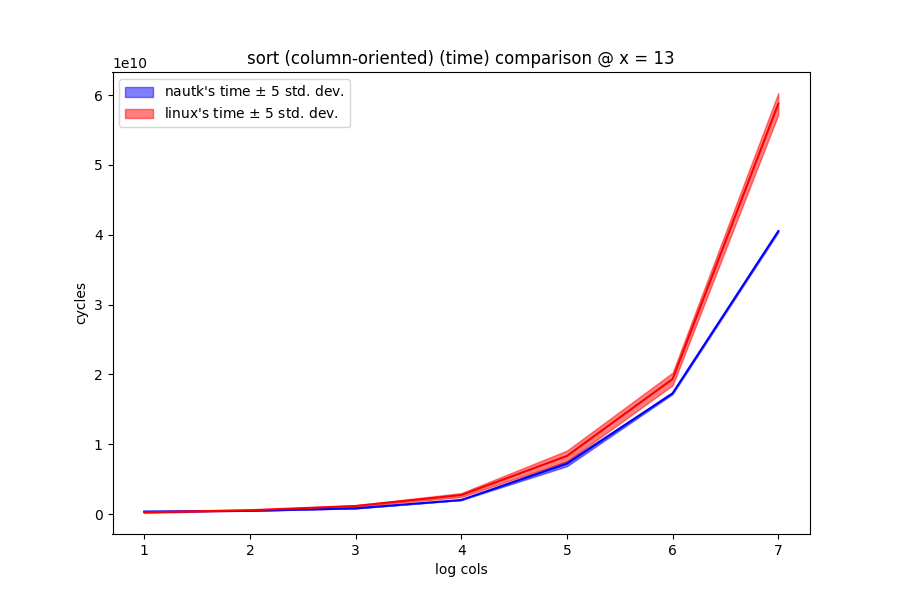
\includegraphics[height=30cm]{plots/sort.png}
  % \todo{for plot: change log cols to cols, increase font size}
  % Unfortunately I do not have the data that this graph was based on anymore. I cannot regenrate it before the deadline.
  \caption{~Column-oriented sort measuring runtime and uncertainty for a fixed chunk size ($8192$), varying the number of columns.}
  \label{fig:sort}
\end{figure}

Nautilus performance is more predictable than Linux, even when its raw performance is worse. Nautilus does not have scheduling interrupts, so it avoids unpredictable detours which also leads to better cache performance (see Table \ref{table:cache_miss-col}).

\begin{table}
  \bgroup
  \def\arraystretch{1.3}%
  \setlength\tabcolsep{1cm}
  \begin{tabular}{l || r | r }
    \textbf{Kernel}    & TLB misses  & Instruction cache misses \\
    \hline\hline
    Linux              & 2,500,000 & 8,200,000 \\
    Nautilus           &         1 & 1,100,000 \\

    % I don't have perf-counter data for the following
    % (there is no perf counter)
    % Page faults              &     & 0 \\
    % Context switches         &     & 0 \\
    % Interrupts               &     & 0 \\
  \end{tabular}
  \egroup
  \caption{~Column-oriented sorting for a $128$ column table with 256 chunks with $8192$ elements each}
  \label{table:cache_miss-col}
\end{table}

%%% Local Variables:
%%% mode: latex
%%% TeX-master: "main"
%%% End:
